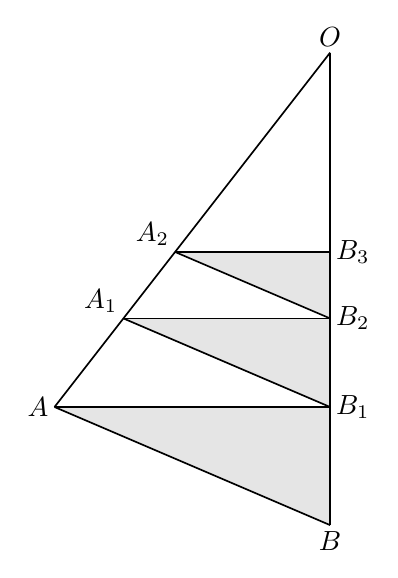
\begin{tikzpicture}[x=1cm,y=1cm,font=\normalsize,
  geometry edge/.style={solid,line width=.6pt,draw=black},
  geometry shade/.style={fill=gray!20,draw=black,line width=.6pt},
  geometry label/.style={font=\normalsize,inner sep=0pt,text=black}]
\coordinate (O) at (4,6);
\coordinate (A) at (0.5,1.5);
\coordinate (A1) at (1.375,2.625);
\coordinate (A2) at (2.03125,3.46875);
\coordinate (B) at (4,0);
\coordinate (B1) at (4,1.5);
\coordinate (B2) at (4,2.625);
\coordinate (B3) at (4,3.46875);
\fill[gray!20] (A)--(B)--(B1)--cycle;
\fill[gray!20] (A1)--(B1)--(B2)--cycle;
\fill[gray!20] (A2)--(B2)--(B3)--cycle;
\draw[geometry edge] (O)--(B);
\draw[geometry edge] (O)--(A);
\draw[geometry edge] (A)--(B);
\draw[geometry edge] (A)--(B1);
\draw[geometry edge] (A1)--(B1);
\draw[geometry edge] (A1)--(B2);
\draw[geometry edge] (A2)--(B2);
\draw[geometry edge] (A2)--(B3);
\node[geometry label,above] at ([yshift=2pt]O) {$O$};
\node[geometry label,left] at ([xshift=-2pt]A) {$A$};
\node[geometry label,above left] at ([xshift=-2pt,yshift=2pt]A1) {$A_{1}$};
\node[geometry label,above left] at ([xshift=-2pt,yshift=2pt]A2) {$A_{2}$};
\node[geometry label,below] at ([yshift=-2pt]B) {$B$};
\node[geometry label,right] at ([xshift=2pt]B1) {$B_{1}$};
\node[geometry label,right] at ([xshift=2pt]B2) {$B_{2}$};
\node[geometry label,right] at ([xshift=2pt]B3) {$B_{3}$};
\end{tikzpicture}
